% 06_p4_data_econ.tex —— P4 数据模型与经济评价（队友；2026-11-20 定稿，
% 含 B1 反事实与增量 NPV）
\section{Problem 4: Data-Driven Production Model and Economic Evaluation}

\subsection{Data Partitioning and Quality Control}
The synthetic production data set (Attachment C) contains 38,880 records:
3 scenarios $\times$ 3 nano-concentrations $\times$ 12 soak-time levels
$\times$ 360 production days, with no missing values and no duplicated rows.
Daily oil rates carry $\pm5\%$ Gaussian noise with non-negative truncation;
truncated (zero) rates occur only in 36 of 108 groups, all in Case~1
(low-permeability) at late production times, and depress $Q_{360}$ by less
than 1--2\%. The bottom-hole pressure decays smoothly from an early maximum
(59.6 MPa in Case~3, briefly above the initial reservoir pressure as the
problem statement allows) and correlates with the oil rate ($\rho = 0.96$),
confirming physical consistency.

Following the blocked cross-validation principle \cite{p4-01}, we partition
by entire (case, $C_n$, $t_s$) groups rather than by individual days:
8 soak levels $\{5,10,20,25,30,35,40,50\}$ d form the training set (72 groups),
$t_s = 55$ d is the validation set, and $t_s \in \{15,45\}$ d (interpolation
hold-out) together with $t_s = 60$ d (extrapolation) form the test set.
The three subsets have no group overlap, and the test set contains soak levels
never seen in training, as required.

\subsection{Production Prediction Models}
We compare four regression models for the group-level cumulative oil
$Q_{360}$: a quadratic response surface, gradient boosting (depth-limited to
3 against over-fitting), random forest, and Gaussian-process (GP) regression
with an RBF kernel; features are $C_n$, $t_s$, their interaction $C_n t_s$,
$\log t_s$, and scenario indicators (the feature set fixed a priori before
any test evaluation). Model selection uses GroupKFold with entire soak levels held
out (8 folds), mirroring the extrapolation task. The GP achieves the best
cross-validated RMSE (25.1 m$^3$ mean, 82.0 worst fold; MAPE 4.6\%) and
validation MAPE of 1.6\%; the tree
ensembles cannot interpolate a withheld interior soak level (their
predictions are piecewise constant in $t_s$), which disqualifies them for the
soak-time scan despite good endpoint behavior. The quadratic surface
under-fits the saturation trend. Simple baselines confirm the need for
nonlinearity: a constant predictor attains 13\% MAPE, a plain linear model
74\%, and a log-$t_s$ linear model 27\%.

The GP is frozen (features and hyper-parameter grid fixed) and evaluated on
the test set exactly once (Table~\ref{tbl:p4_test}): MAPE is 0.53\% on the
interpolation hold-out and 3.59\% on the $t_s = 60$ d extrapolation, well
within the 15\% target, with rank correlation above 0.98 everywhere.

\begin{table}[h!t]
\centering
\caption{Frozen GP: one-shot test performance for $Q_{360}$.}
\label{tbl:p4_test}
\small
\begin{tabular}{lccccc}
\toprule[1.5pt]
Subset & $n$ & RMSE (m$^3$) & MAPE (\%) & Spearman\\
\midrule[1pt]
Interpolation ($t_s=15/45$) & 18 & 11.6 & 0.53 & 1.000\\
Extrapolation ($t_s=60$)    & 9  & 26.6 & 3.59 & 0.983\\
\bottomrule[1.5pt]
\end{tabular}
\end{table}

Prediction uncertainty is quantified with the GP posterior std. Out-of-fold
95\% intervals cover 94.4\% of training groups (nominal 95\%), so the raw
posterior is close to calibrated; a variance-scaling calibration
($\kappa = 0.47$) degrades coverage to 80.6\% and is therefore not adopted.
On the test set the coverage is 92.6\%, reflecting honestly widened
intervals under extrapolation. Interpretability analysis (permutation
importance and partial-dependence
plots) attributes 74\% of predictive power to the scenario indicators
(permeability contrast between cases), 20\% to the soak time, and only
6\% to the nano-concentration within the studied range; the partial-dependence
curves show $Q_{360}$ increasing near-linearly in $C_n$ and saturating in
$t_s$, consistent with the $\sqrt{t}$ pressure-diffusion scaling of the
mechanistic model (Section~4).

\subsection{Economic Evaluation under Appendix B}
The economic module strictly follows Appendix~B: all volumes are metered at
the 25 MPa, 300 K reference state; $t_{inj} = V_{inj}/q_{inj}$; cash flows
are discounted daily at $r = 8\%$/yr from day 0; the injection fee accrues
over the actual injection days, the soak fee over $t_s$, and the production
phase carries only variable costs ($c_{prod} = 0.035$, $c_{water} = 0.0025$
10$^4$ CNY/m$^3$). The implementation reproduces the worked example of the
problem statement to the cent (848.25$\times10^4$ CNY for
$V_{inj}=3000$ m$^3$, $f_{CO_2}=0.5$, $C_n=1.0$ wt\%, 10 d injection and
30 d soak). Produced-water data are absent from Attachment~C (a known data
gap); we adopt a water--oil ratio $WOR = 0.5$ and show that NPV varies by
less than 2\% over $WOR \in [0,2]$.

Figure~\ref{fig:p4_npv} shows NPV versus soak time for the three scenarios
at the baseline operation ($q_{inj}=300$ m$^3$/d, $V_{inj}=3000$ m$^3$,
$f_{CO_2}=0.5$, $\tau_{inj}=0$). The economically optimal soak time
(maximizing NPV) is $t_s^* = 10$ d for Case~1, 20--25 d for Case~2, and
30--40 d for Case~3 (35 d at $C_n=1.0$). Only Case~3 attains a positive
absolute NPV (up to $+284\times10^4$ CNY at $C_n=0.5$, $t_s=40$ d);
Case~1 and Case~2 remain negative at all soak levels because the 3000 m$^3$
fluid slug dwarfs the producible volume---a conclusion independently
supported by the injectivity analysis of the mechanistic model, which shows
Case~1 cannot even accept 300 m$^3$/d without exceeding $p_{max}$
(Section~5). Breakeven oil prices at $t_s^*$ are 796 USD/bbl (Case~1),
157 USD/bbl (Case~2) and 64 USD/bbl (Case~3, below the 75 USD/bbl market
price), i.e.\ Case~3 is the only economically viable scenario under the
baseline operation. Following the requirement to report loss categories
separately, we distinguish (i) engineering infeasibility (violation of
$p_{max}$, handled as a hard constraint in Section~5), (ii) absolute
NPV $<0$ (all 36 Case~1 and Case~2 combinations tested, 6 of 36 in
Case~3), and (iii) $\Delta NPV = NPV - NPV_{B1}$ against the
fracturing-only baseline $B1$.

\paragraph{Fracturing-only counterfactual.}
For $B1$, production starts from the initial pressure and saturations,
with no injection or soak. We retain the fracture geometry, well-pressure
and liquid limits, and use the tank decline with the case-specific
storage length from the $C_n=1.0$~wt\%, $t_s=30$~d training fit.
The same $WOR=0.5$ is used. Over 360~d, only the initial fracturing
cost and variable production and water costs are charged.
For Cases~1--3, respectively, $NPV_{B1}$ is $-33.58$, $280.47$ and $915.97$
in units of $10^4$~CNY. At each case's best reference-operation combination
(all at $C_n=0.5$~wt\%), $\Delta NPV$ is $-539.55$, $-595.40$ and $-632.45$
in the same units. Case~3 has positive absolute NPV and negative
incremental NPV under this storage-length assumption. Attachment~C
contains no fracturing-only production series, so these incremental
values depend on the counterfactual storage model. In Case~3 the incremental NPV changes sign at a B1 storage length of about 0.176~m under the same rate and cost assumptions \cite{codex}.

\subsection{Mechanism--Data Comparison}
Figure~\ref{fig:p4_overlay} overlays the frozen-GP $Q_{360}(t_s)$ curves
on the observed group means at $C_n = 1.0$ wt\%. Two viewpoints on the
optimal soak time emerge, as anticipated in the master plan. The
\emph{production} viewpoint defines $t_s^*$ as the inflection point of the
cumulative-production-increment curve \cite{p4-04}, which the GP curves
place at the earliest scanned level (5~d) in all three scenarios---the
increment decays monotonically from the start. The \emph{economic}
viewpoint of \S6.3 instead yields interior optima (10/20/35~d at $C_n=1$~wt\%), because
daily discounting and the soak-day fee shift the optimum to shorter
soaks; the two definitions are both reported and their divergence is
explained by the time-budget difference, not by physics
\cite{p4-04, p4-05}.

Three effects limit the mechanism--data comparison.
\emph{Model assumptions:} the tank model uses a fixed calibrated storage
length in its independent Case~3 check. Its cumulative error is 5.36\% at
55~d, and it misses the observed gain from 30 to 55~d. Local damage tests
at prescribed pressure histories yield $d=0$ at the nominal thresholds.
\emph{Numerical error:} at the 0.01~wt\% threshold the calculated nano
radius changes from zero with 50 cells to 0.15~m with 200 cells in the
Case~3 injection test. The radius remains grid-dependent.
\emph{Data noise:} Attachment~C contains synthetic daily variability.
The within-group rate CV also includes the production decline, so the
decline and noise are treated separately when interpreting the residuals.
Figure~\ref{fig:p4_overlay} compares the frozen data model with Attachment~C.

\begin{figure}[h!t]
\centering
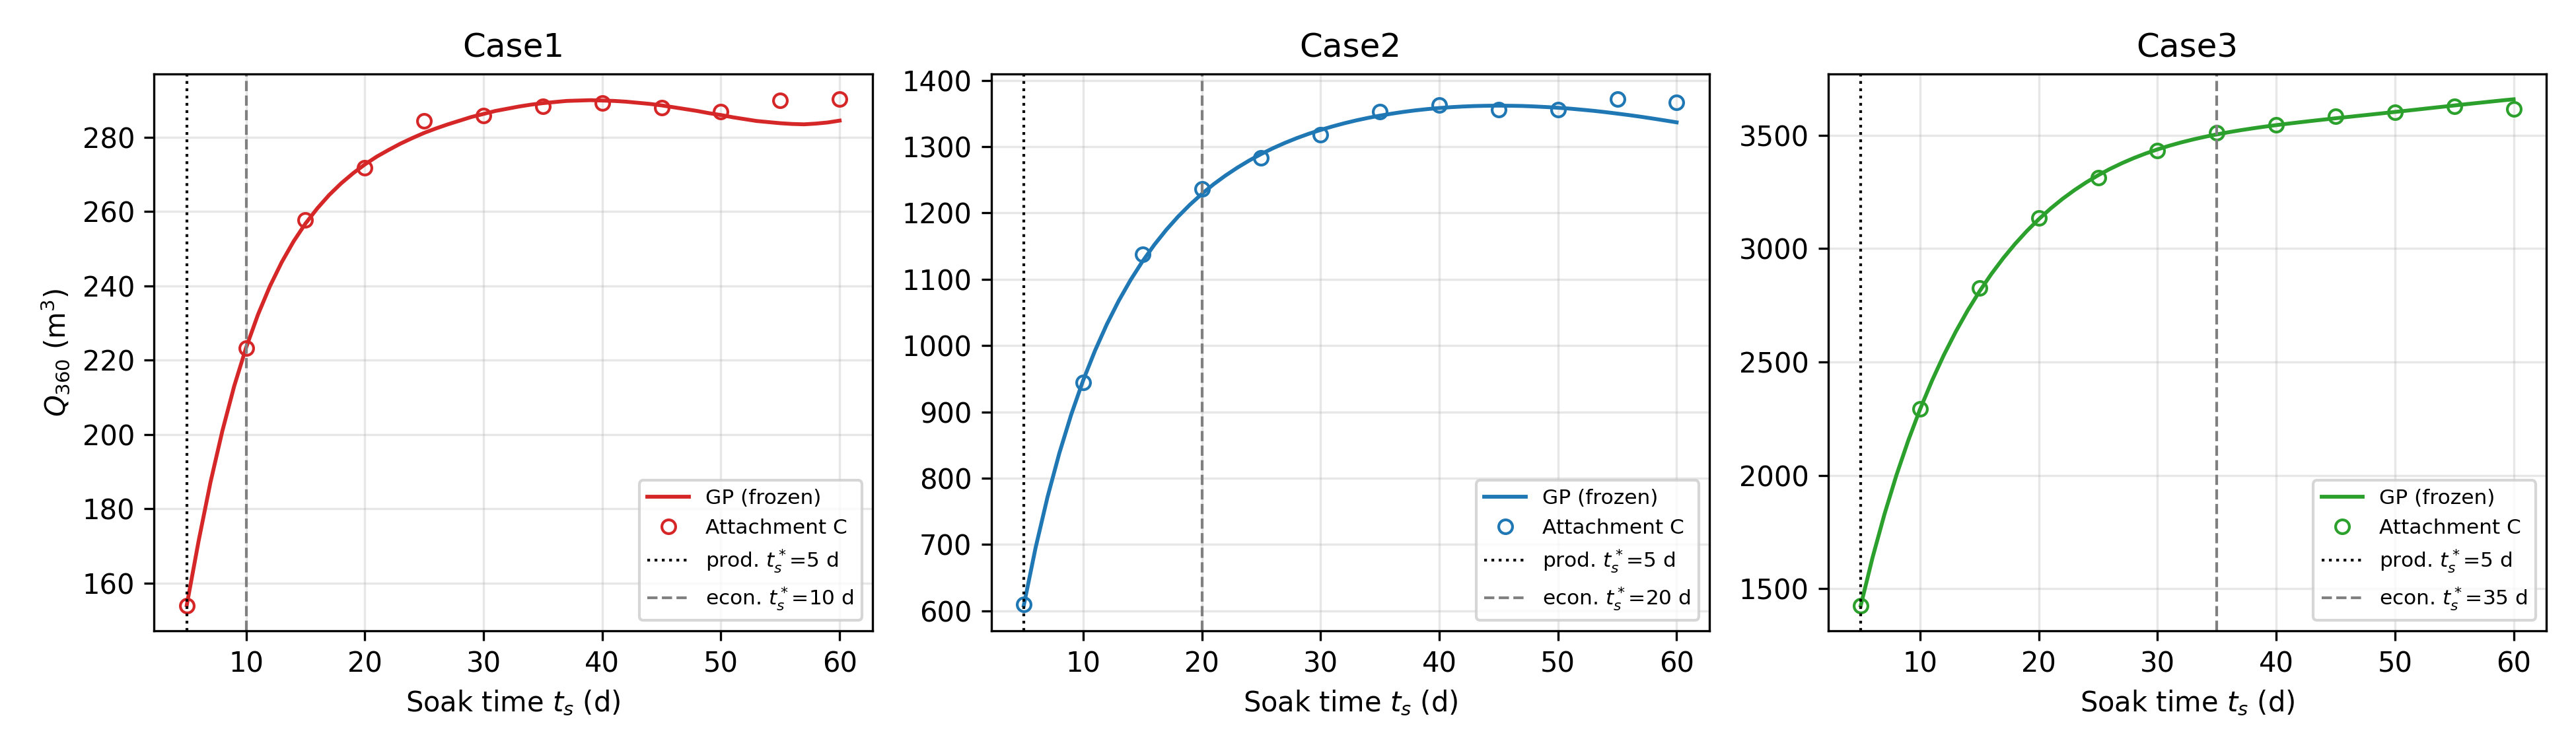
\includegraphics[width=\textwidth]{p4_mech_data.png}
\caption{Frozen-GP production curves $Q_{360}(t_s)$ (lines) versus
observed group means (circles) at $C_n = 1.0$ wt\%; economic-optimum
soak levels (ticks) are interior while production-increment inflection
occurs at the earliest level.}
\label{fig:p4_overlay}
\end{figure}

% 图表（T36/T37 定稿统一编号）：
%   fig:p4_split   T03_split_overview.png      数据划分
%   fig:p4_models  T12_model_comparison.png    模型对比 + val 散点
%   fig:p4_npv     T16_npv_ts_curves.png       NPV–ts 曲线
%   fig:p4_interpret T15_interpretability.png  重要性 + PDP

\begin{figure}[h!t]
\centering
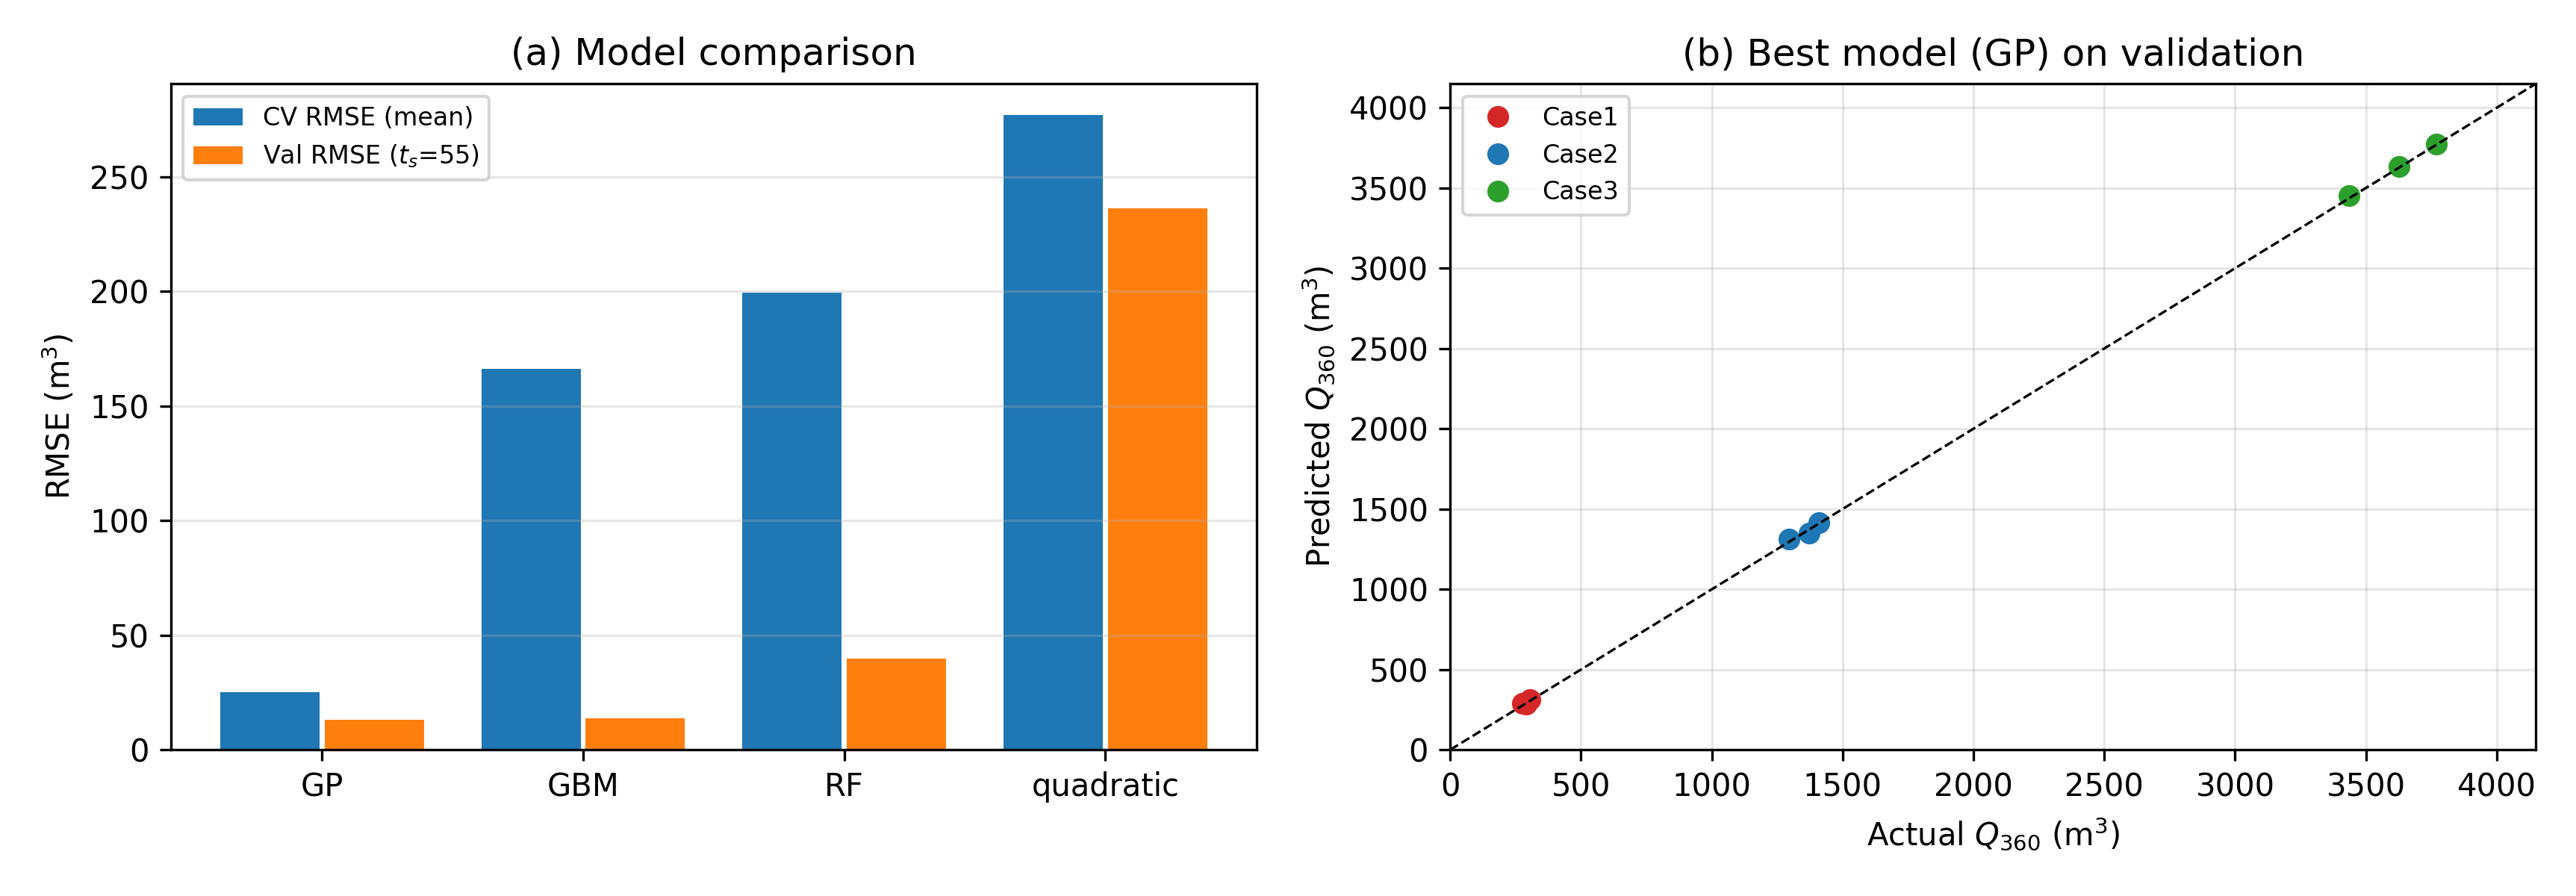
\includegraphics[width=0.9\textwidth]{p4_model_comp.png}
\caption{Model comparison for $Q_{360}$ (GroupKFold by soak level): the
GP dominates; tree ensembles fail to interpolate withheld interior soak
levels; baselines confirm the need for nonlinear features.}
\label{fig:p4_models}
\end{figure}

\begin{figure}[h!t]
\centering
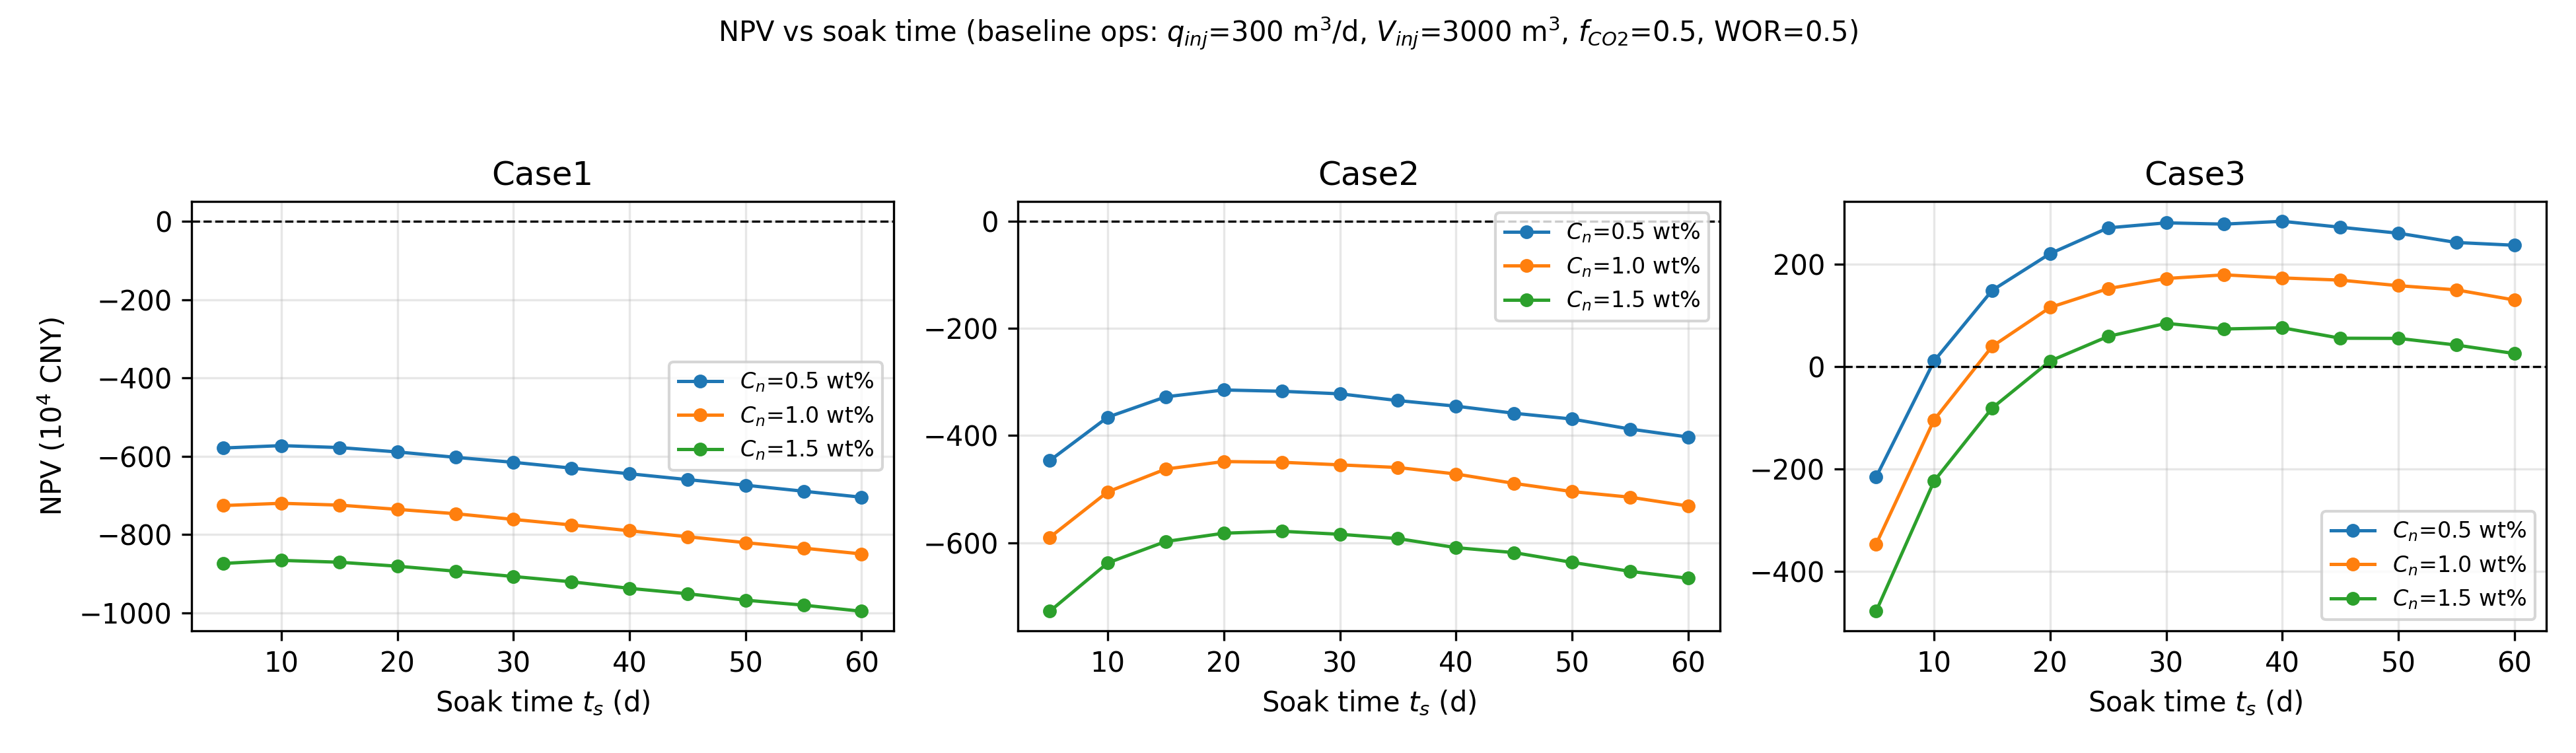
\includegraphics[width=0.9\textwidth]{p4_npv_ts.png}
\caption{NPV versus soak time at baseline operation; interior economic
optima in all scenarios, positive NPV only in Case~3.}
\label{fig:p4_npv}
\end{figure}

\begin{figure}[h!t]
\centering
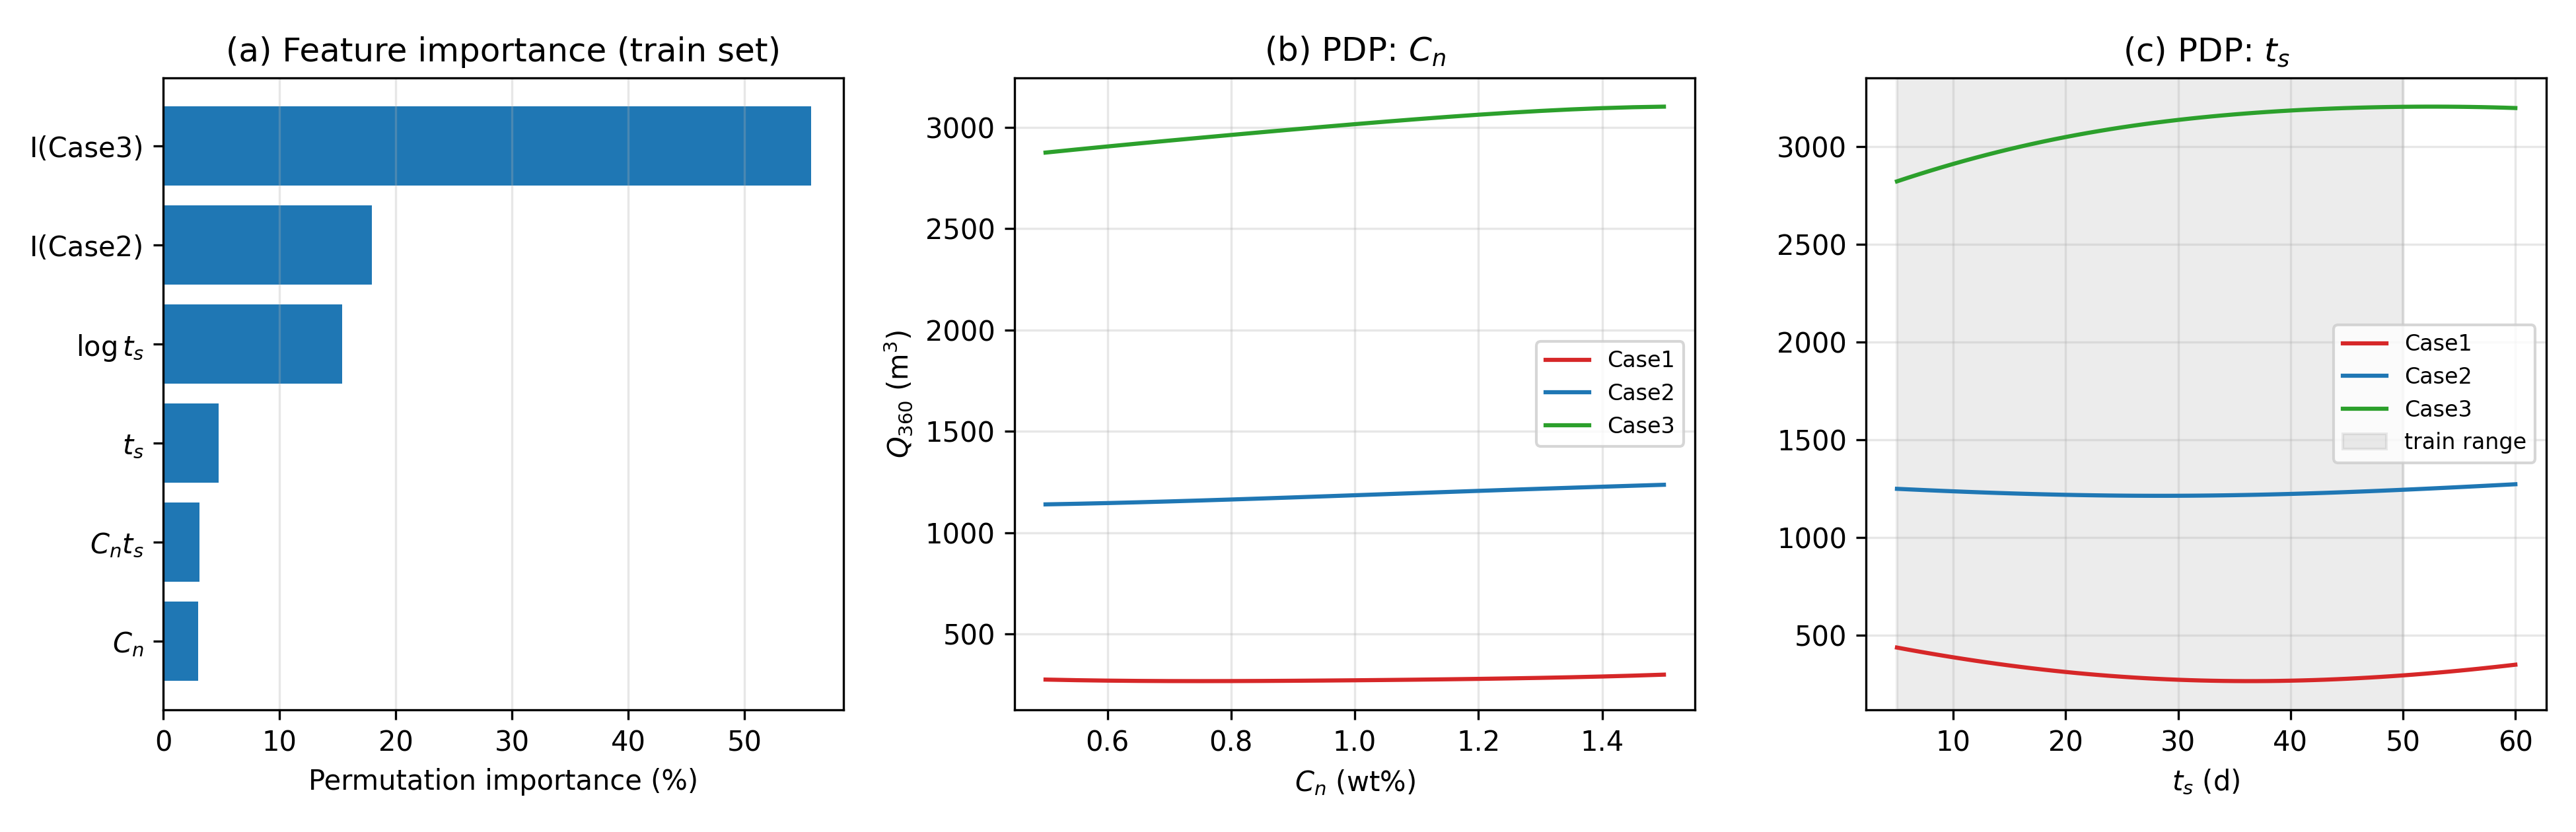
\includegraphics[width=0.9\textwidth]{p4_importance.png}
\caption{Permutation importance and partial-dependence profiles of the
frozen GP; scenario identity dominates, $C_n$ contributes least.}
\label{fig:p4_interpret}
\end{figure}
